% ============================================================
% QUDA MultiGrid 理解与 PyQCU 复现 — 学术成果展示
% 编译：xelatex 两遍；交付闸门：Overfull=0, Float too large=0
% ============================================================
\documentclass[UTF8,aspectratio=169,11pt]{ctexbeamer}

\usepackage{amsmath,amssymb}
\usepackage{booktabs}
\usepackage{tabularx}
\usepackage{array}
\usepackage{tikz}
\usetikzlibrary{arrows.meta,positioning,calc,fit,shapes.geometric}
\usepackage{listings}
\usepackage{xcolor}
\usepackage{microtype}
\usepackage{hyperref}

\definecolor{primary}{HTML}{17365D}
\definecolor{accent}{HTML}{1F77B4}
\definecolor{evidence}{HTML}{1E8449}
\definecolor{warning}{HTML}{C55A11}
\definecolor{muted}{HTML}{5B6573}
\definecolor{panel}{HTML}{F4F7FA}
\definecolor{linegray}{HTML}{CBD5E1}
\definecolor{violet}{HTML}{6C4A9E}
\definecolor{good}{HTML}{EAF5EE}
\definecolor{warnbg}{HTML}{FFF4E8}

\setbeamersize{text margin left=0.55cm,text margin right=0.55cm}
\setlength{\columnsep}{0.34cm}
\setlength{\emergencystretch}{2em}
\setbeamertemplate{navigation symbols}{}
\setbeamertemplate{blocks}[rounded][shadow=false]
\setbeamercolor{normal text}{fg=black!86,bg=white}
\setbeamercolor{structure}{fg=primary}
\setbeamercolor{frametitle}{fg=primary,bg=white}
\setbeamercolor{block title}{fg=primary,bg=panel}
\setbeamercolor{block body}{fg=black!86,bg=panel}
\setbeamercolor{alerted text}{fg=warning}
\setbeamerfont{frametitle}{size=\large,series=\bfseries}
\setbeamerfont{normal text}{size=\normalsize}
\setbeamertemplate{frametitle}{\vskip0.12cm\insertframetitle\par\vskip0.08cm}
\setbeamertemplate{footline}{%
  \hbox{\begin{beamercolorbox}[wd=\paperwidth,ht=2.3ex,dp=0.9ex,
    leftskip=0.55cm,rightskip=0.55cm]{author in head/foot}%
    \scriptsize\color{muted}\insertshortauthor\hfill
    \insertshorttitle\hfill\insertframenumber/\inserttotalframenumber
  \end{beamercolorbox}}}

\newcolumntype{Y}{>{\raggedright\arraybackslash}X}
\newcolumntype{P}[1]{>{\raggedright\arraybackslash}p{#1}}
\newcommand{\source}[1]{%
  \vspace{0.02em}\par{\raggedright\fontsize{5.5pt}{6.5pt}\selectfont\color{muted}来源：#1\par}}
% 在公式中也允许引用代码路径；先 detokenize，避免参数中的下划线被当作下标。
\newcommand{\codepath}[1]{%
  \ifmmode\text{\ttfamily\detokenize{#1}}%
  \else\texttt{\detokenize{#1}}\fi}
\newcommand{\verified}{\textcolor{evidence}{确证}}
\newcommand{\inferred}{\textcolor{accent}{推断}}
\newcommand{\unverified}{\textcolor{warning}{未验证}}
\newcommand{\risk}{\textcolor{warning}{风险}}
\newcommand{\passmark}{\textcolor{evidence}{PASS}}

\tikzset{
  flow/.style={draw=accent,fill=accent!8,rounded corners=2pt,align=center,
    minimum height=0.64cm,text width=2.05cm,font=\small},
  state/.style={draw=primary,fill=primary!7,rounded corners=2pt,align=center,
    minimum height=0.62cm,text width=2.42cm,font=\small},
  phase/.style={draw=violet,fill=violet!8,rounded corners=2pt,align=center,
    minimum height=0.58cm,text width=2.16cm,font=\small},
  decision/.style={draw=warning,fill=warning!10,diamond,aspect=2.0,align=center,
    inner sep=1.2pt,font=\small},
  arrow/.style={-{Latex[length=2mm]},draw=primary,semithick},
  relation/.style={-{Latex[length=1.7mm]},draw=muted,thin,dashed},
  labelstyle/.style={font=\scriptsize,inner sep=1.5pt,fill=white,text=muted}
}

\lstset{
  basicstyle=\ttfamily\scriptsize,
  backgroundcolor=\color{panel},frame=single,
  breaklines=true,breakatwhitespace=false,keepspaces=true,
  columns=flexible,numbers=left,numberstyle=\tiny\color{muted},
  keywordstyle=\color{primary}\bfseries,
  commentstyle=\color{evidence!70!black},stringstyle=\color{accent}
}

\title[QUDA MG 复现]{QUDA MultiGrid 的算法理解与 PyQCU 复现}
\subtitle{P/R 聚合、Galerkin 粗化、Clover/Gauge、Schur 奇偶与递归预条件}
\author[代码审计与代数验证]{代码审计与代数验证}
\institute{PyQCU · Lattice QCD}
\date{2026 年 8 月 29 日}

\begin{document}

\begin{frame}[plain]
  \titlepage
\end{frame}

\begin{frame}[t]{结论先行：QUDA 的代数主线已落到 PyQCU 参考实现}
  \small
  \begin{columns}[T,totalwidth=\textwidth]
    \begin{column}{0.30\textwidth}
      \begin{block}{已完成}
        新增独立的 \codepath{QudaTransfer}、\codepath{QudaCoarseOperator}、\codepath{ParitySchurOperator} 与 \codepath{QudaMultigrid}；旧 \codepath{multigrid} 原样保留。
      \end{block}
    \end{column}
    \begin{column}{0.30\textwidth}
      \begin{block}{直接证据}
        CPU、$4^4$、复数单精度回归 \passmark{}：\textbf{9 passed}。实测 $RP$、伴随、Galerkin、Schur 重构和 full residual 均达到 $10^{-6}$--$10^{-7}$ 量级。
      \end{block}
    \end{column}
    \begin{column}{0.30\textwidth}
      \begin{alertblock}{边界}
        这是可验证的 Python 参考路径，不是 QUDA 生产 GPU kernel。CUDA/MPI halo、NVSHMEM、完整 setup Krylov 与硬件性能仍 \unverified{}。
      \end{alertblock}
    \end{column}
  \end{columns}
  \vspace{0.35em}
  \begin{center}
    \begin{tikzpicture}[node distance=0.20cm and 0.22cm]
      \node[flow] (b) {近零模\\$B_\ell$};
      \node[flow,right=of b] (v) {局部基\\$V_\ell$};
      \node[flow,right=of v] (pr) {延拓/限制\\$P_\ell,R_\ell$};
      \node[flow,right=of pr] (dc) {粗算子\\$D_{\ell+1}=RDP$};
      \node[flow,right=of dc] (mg) {Schur +\\递归 cycle};
      \draw[arrow] (b)--(v)--(pr)--(dc)--(mg);
    \end{tikzpicture}
  \end{center}
  \vspace{0.18em}
  \begin{tabular}{@{}p{0.94\textwidth}@{}}
    \colorbox{good}{\parbox{0.905\textwidth}{\textbf{阶段判断：}\quad 已经复现 QUDA 的核心代数对象与奇偶路径；下一阶段才是把 reference operator 替换成批量 kernel、MPI halo 和真实大格求解器。}}
  \end{tabular}
  \source{实现：\codepath{pyqcu/solver/_quda_multigrid.py:188-1407}；测试：\codepath{examples/pyqcu/test_quda_multigrid.py:56-264}；本次命令：\codepath{pytest -q examples/pyqcu/test_quda_multigrid.py}。}
\end{frame}

\begin{frame}[t]{第一性原理：smoother 消高频，粗空间承接长程误差}
  \footnotesize
  \begin{columns}[T,totalwidth=\textwidth]
    \begin{column}{0.45\textwidth}
      \begin{block}{误差分解与 Galerkin 投影}
        设 $e=e_{\rm high}+e_{\rm low}$。局部平滑器快速削弱 $e_{\rm high}$，而慢变的 $e_{\rm low}$ 由近零模张成的粗空间表示：
        \begin{align*}
          e_{\rm low}&\simeq P e_c, &
          e_c&\simeq (RDP)^{-1}Rr,\\
          D_c&=RDP, & R&=P^\dagger .
        \end{align*}
      \end{block}
      \begin{block}{不变量}
        $P^\dagger P=I_c$（局部 aggregate 意义）；$D_c$ 的 native apply 必须与显式 $P\to D\to R$ 相同。
      \end{block}
    \end{column}
    \begin{column}{0.45\textwidth}
      \begin{tikzpicture}[node distance=0.38cm and 0.36cm]
        \node[phase] (h) {局部高频\\误差};
        \node[phase,right=of h] (s) {MR/GCR\\smoother};
        \node[phase,below=of h] (l) {长程低频\\误差};
        \node[phase,right=of l] (p) {近零模\\$P/R$ 粗化};
        \node[decision,below=of s] (c) {真残差\\是否达标？};
        \draw[arrow] (h)--(s);
        \draw[arrow] (l)--(p);
        \draw[relation] (s)--(c);
        \draw[relation] (p)--(c);
        \draw[relation] (c.west) |- ++(-0.65,0) |- node[left=1pt,labelstyle]{否：再迭代} (h.west);
      \end{tikzpicture}
      \vspace{0.5em}
      \begin{alertblock}{物理检查}
        规范场 $U_\mu$、Clover 局部项 $C$ 和 hopping 共同定义 $D$；不能只把 hopping 粗化而丢掉 local term，否则 Schur 与粗层物理算子不一致。
      \end{alertblock}
    \end{column}
  \end{columns}
  \source{QUDA 算法入口：\codepath{refer/git-rep/quda/lib/multigrid.cpp:72-197,1131-1224}；Galerkin/验证：\codepath{refer/git-rep/quda/lib/coarse_op.cuh:1035-1459}、\codepath{refer/git-rep/quda/lib/multigrid.cpp:783-1069}。}
\end{frame}

\begin{frame}[t]{层级 setup：每层都是 Transfer + coarse Dirac + 两侧平滑 + 粗解器}
  \small
  \begin{columns}[T,totalwidth=\textwidth]
    \begin{column}{0.57\textwidth}
      \begin{tabular}{@{}l@{}}
        $\text{输入： }(D_\ell,B_\ell,\;b_\ell,\;\text{geometry},\;\text{precision})$\\
        $\text{1. map： }a(x)=\lfloor x/b\rfloor,\quad\text{建立 fine/coarse 索引}$\\
        $\text{2. transfer： }B_\ell\xrightarrow{\text{aggregate CGS}}V_\ell\xrightarrow{}(P_\ell,R_\ell)$\\
        $\text{3. coarse： }D_{\ell+1}=R_\ell D_\ell P_\ell\xrightarrow{}(X_\ell,Y_\ell)$\\
        $\text{4. PC： }X_\ell^{-1},\;Yhat_\ell\xrightarrow{}\text{even/odd Schur}$\\
        $\text{5. recurse： }B_{\ell+1}\text{ 与下一层}\;D_{\ell+1}\text{；底层接 Krylov}$\\
        $\text{输出： }\text{pre/post smoother}+\text{coarse solver}+\text{level state}$
      \end{tabular}
    \end{column}
    \begin{column}{0.37\textwidth}
      \begin{block}{QUDA 的构造顺序}
        \begin{tikzpicture}[node distance=0.08cm]
          \node[state,text width=2.45cm,minimum height=0.48cm,font=\scriptsize] (a) {细格 Dirac / smoother};
          \node[state,text width=2.45cm,minimum height=0.48cm,font=\scriptsize,below=of a] (b) {B：加载、随机或 setup solver};
          \node[state,text width=2.45cm,minimum height=0.48cm,font=\scriptsize,below=of b] (c) {Transfer 与 $RDP$ coarse op};
          \node[state,text width=2.45cm,minimum height=0.48cm,font=\scriptsize,below=of c] (d) {$X^{-1}$、$Yhat$、下一层};
          \node[state,text width=2.45cm,minimum height=0.48cm,font=\scriptsize,below=of d] (e) {solver wrapper / cycle};
          \draw[arrow] (a)--(b)--(c)--(d)--(e);
        \end{tikzpicture}
      \end{block}
      \begin{block}{PyQCU 对应}
        \scriptsize\codepath{setup()} 建立 \codepath{levels/transfers}；\codepath{v_cycle()} 返回校正。
      \end{block}
    \end{column}
  \end{columns}
  \vspace{-0.60em}
  \source{QUDA：\codepath{multigrid.cpp:72-434,564-702}；PyQCU：\codepath{_quda_multigrid.py:986-1211}；图为控制流抽象。}
\end{frame}

\begin{frame}[t]{P/R 的核心是同一套几何 map 与 spin/parity map}
  \footnotesize
  \begin{columns}[T,totalwidth=\textwidth]
    \begin{column}{0.44\textwidth}
      \begin{block}{几何与自旋映射}
        \begin{align*}
          a(x)&=\left(\left\lfloor\frac{x_0}{b_0}\right\rfloor,\ldots,\left\lfloor\frac{x_3}{b_3}\right\rfloor\right),\\
          q(s,p)&=\begin{cases}
            \lfloor s/b_s\rfloor,&\text{Wilson/Clover},\\
            p(x),&\text{staggered }(b_s=0).
          \end{cases}
        \end{align*}
        Wilson/Clover 典型为 $4\to2$ spin、$b_s=2$；staggered 为 $1\to2$，粗 spin 承载 checkerboard parity。
      \end{block}
      \begin{block}{维数}
        $D_f=4\times3=12$；粗层 $D_c=2\times N_{\rm vec}$。\codepath{dof_list=[12,24,24]} 解释为每层总 DOF，而不是每个 coarse-spin block 的向量数。
      \end{block}
    \end{column}
    \begin{column}{0.46\textwidth}
      \begin{block}{$P$ 与 $R$}
        对每个 aggregate $a$ 和 coarse spin $q$，$V_{s,c,q,j}(x)$ 是局部正交列：
        \begin{align*}
          (P\eta)_{s c}(x)&=\sum_j V_{s c q j}(x)\eta_{qj}(a(x)),\\
          (R\psi)_{qj}(a)&=\sum_{x\in a,,s,c}V^*_{s c q j}(x)\psi_{s c}(x).
        \end{align*}
        因而 $R=P^\dagger$；$RP\eta\simeq\eta$ 是最先应测的不变量。
      \end{block}
      \begin{tikzpicture}[node distance=0.18cm and 0.12cm]
        \node[flow,text width=1.86cm,minimum height=0.52cm,font=\scriptsize] (f) {细 block\\$b_0\times b_1\times b_2\times b_3$};
        \node[flow,text width=1.86cm,minimum height=0.52cm,font=\scriptsize,right=of f] (a) {粗 site\\$a(x)$\\+ coarse spin $q$};
        \node[flow,text width=1.86cm,minimum height=0.52cm,font=\scriptsize,right=of a] (c) {粗 color\\$j=1,\ldots,N_{\rm vec}$};
        \draw[arrow] (f)--node[above=1pt,labelstyle]{$P$}(a);
        \draw[arrow] (a)--node[above=1pt,labelstyle]{$R=P^\dagger$}(c);
      \end{tikzpicture}
    \end{column}
  \end{columns}
  \source{QUDA：\codepath{transfer.cpp:200-328}；PyQCU：\codepath{_quda_multigrid.py:197-460}。}
\end{frame}

\begin{frame}[t]{块 CGS：正交对象是 aggregate-local 的列，而不是全局向量}
  \footnotesize
  \begin{columns}[T,totalwidth=\textwidth]
    \begin{column}{0.55\textwidth}
      \begin{tabular}{@{}l@{}}
        $\text{for each aggregate }a\text{ and coarse spin }q:$\\
        \quad $\text{load }v_j\leftarrow B_j\;(\text{首轮})\text{ 或 }V_j\;(\text{后续轮})$\\
        \quad $h_{ij}=\langle v_i,v_j\rangle_{a,q},\qquad v_j\leftarrow v_j-h_{ij}v_i$\\
        \quad $v_j\leftarrow v_j/\|v_j\|_{a,q}\quad(\text{逐列归一化})$\\
        \quad $j=0,\ldots,N_{\rm vec}-1$\\
        $\text{repeat }n_{\rm block\_ortho}\text{ passes}$\\
        $\text{return }V\text{；再以同一 }V\text{ 定义 }P,R$
      \end{tabular}
      \vspace{0.10em}
      \begin{block}{容量约束}
        $N_{\rm vec}\le N_c\,|a|\,b_s$（Wilson/Clover）；staggered 有效容量为 $N_c|a|/2$。超出局部维数时只能得到零列/相关列。
      \end{block}
    \end{column}
    \begin{column}{0.35\textwidth}
      \begin{block}{源码对应}
        QUDA kernel 按 aggregate、parity、chirality 和 vector tile 并行；首轮从 $B$ 读，之后从 $V$ 读，最后归一化保存。
      \end{block}
      \begin{block}{PyQCU 复现}
        \codepath{_cg_orthogonalise()} 使用复数 CGS，逐 block 批量执行；\codepath{_block_orthogonalise()} 分别处理 Wilson/Clover 与 staggered slow path。
      \end{block}
      \begin{alertblock}{验证}
        实测 block-ortho 最大 Gram 误差：$5.34\times10^{-7}$（多层例），staggered：$3.38\times10^{-7}$。
      \end{alertblock}
    \end{column}
  \end{columns}
  \vspace{-0.35em}
  \source{QUDA：\codepath{block_orthogonalize.cuh:149-239}、\codepath{transfer.cpp:152-163}；PyQCU：\codepath{_quda_multigrid.py:155-185,285-351}。}
\end{frame}

\begin{frame}[t]{粗算子保留 local Clover 与 Gauge hopping：$D_c=RDP$}
  \footnotesize
  \begin{columns}[T,totalwidth=\textwidth]
    \begin{column}{0.43\textwidth}
      \begin{block}{动作形式}
        {\scriptsize
        \begin{align*}
          D_c\eta(q)&=X(q)\eta(q)+\sum_{\mu=0}^{3}\big[ Y^+_\mu(q)\eta(q+\hat\mu)\\[-0.2em]
          &\qquad+Y^-_\mu(q)\eta(q-\hat\mu)\big].
        \end{align*}}
        $X$ 是目标点 local block；$Y^\pm$ 是 coarse link。周期边界与邻居坐标必须和 \codepath{...xyzt} 布局一致。
      \end{block}
      \begin{block}{物理来源}
        细格 $D(U,C,\kappa)$ 经 $V^\dagger D V$ 投影：hopping 贡献 $V^\dagger U_\mu V$，Clover/local 贡献 $V^\dagger C V$；无 Clover 时保留 identity/local diagonal。
      \end{block}
    \end{column}
    \begin{column}{0.47\textwidth}
      \begin{tabular}{@{}P{0.22\linewidth}P{0.67\linewidth}@{}}
        \toprule
        对象 & QUDA 与 PyQCU 的对应 \\
        \midrule
        QUDA $Y$ & UV 后再 VUV，按 forward/backward、dimension 累加，必要时双向 link 与 halo \\
        QUDA $X$ & coarse Clover/local field；coarse-on-coarse 仍按 $V^\dagger C V$ 组织 \\
        PyQCU materialize & 逐粗自由度 probe：$P\to D\to R$，按 displacement 聚成 block \\
        PyQCU lazy & 每次直接执行 $R(D(P\eta))$；避免大格显式矩阵 \\
        \bottomrule
      \end{tabular}
      \vspace{0.10em}
      \begin{alertblock}{边界修正}
        粗 extent 为 2 时 $+\hat\mu$ 与 $-\hat\mu$ 是同一邻点；实现将两份方向系数各折半，避免 apply 重复计数。
      \end{alertblock}
    \end{column}
  \end{columns}
  \source{QUDA：\codepath{coarse_op.cuh:1040-1459}、\codepath{dirac_coarse.cpp:121-239}；PyQCU：\codepath{_quda_multigrid.py:573-805}。}
\end{frame}

\begin{frame}[t]{Clover、Gauge 和粗层算子：接口不同，代数对象相同}
  \footnotesize
  \begin{columns}[T,totalwidth=\textwidth]
    \begin{column}{0.47\textwidth}
      \begin{block}{PyQCU 细层入口}
        \begin{tabular}{@{}l@{}}
          $U\;[3,3,4,X,Y,Z,T]$\\
          $C\;[4,3,4,3,X,Y,Z,T]\quad(\text{可选})$\\
          $\downarrow\quad$\codepath{dslash.operator(U,C,kappa)}\\
          $D_f\;[12,X,Y,Z,T],\quad X_f=I\text{ 或 }M_C$
        \end{tabular}
        \vspace{0.25em}
        无 Clover 时细层 diagonal 是 identity；有 Clover 时取 \codepath{operator.sitting.M}。这使 parity Schur 总能调用局部逆。
      \end{block}
      \begin{block}{粗层递归}
        第一层得到 $D_1=R_0D_0P_0$；下一层把 $D_1$ 作为新的 fine operator，再用 $B_1$、$P_1/R_1$ 继续粗化。
      \end{block}
    \end{column}
    \begin{column}{0.43\textwidth}
      \begin{block}{QUDA 细节}
        \scriptsize
        \begin{minipage}{\linewidth}
          \codepath{createY()}：粗 link $Y$ 与 local $X$；\\[-0.1em]
          \codepath{createCoarseOp()}：aggregate-only 粗化；\\[-0.1em]
          \codepath{DiracCoarsePC}：以 $Yhat+X$ 施加 PC hopping；\\[-0.1em]
          coarse-on-coarse：$C$ 进入下一次 VUV/local。
        \end{minipage}
      \end{block}
      \begin{tikzpicture}[node distance=0.10cm and 0.14cm]
        \node[flow,text width=1.38cm,minimum height=0.44cm,font=\scriptsize] (u) {Gauge $U$};
        \node[flow,text width=1.38cm,minimum height=0.44cm,font=\scriptsize,right=of u] (c) {Clover $C$};
        \node[flow,text width=1.38cm,minimum height=0.44cm,font=\scriptsize,below=of u] (d) {细层 $D_f$};
        \node[flow,text width=1.38cm,minimum height=0.44cm,font=\scriptsize,right=of d] (g) {$R D_f P$};
        \draw[arrow] (u)--(d);
        \draw[arrow] (c)--(d);
        \draw[arrow] (d)--(g);
      \end{tikzpicture}
      \vspace{0.3em}
      \begin{alertblock}{当前实现级别}
        \verified{} 代数检查通过；\unverified{} CUDA 侧 UV/VUV、field order、ghost exchange 尚未迁移。
      \end{alertblock}
    \end{column}
  \end{columns}
  \source{PyQCU：\codepath{_quda_multigrid.py:1003-1116}；QUDA：\codepath{dirac_coarse.cpp:121-626}。}
\end{frame}

\begin{frame}[t]{预条件粗算子：先消去 even，再在 odd Schur 上求解}
  \small
  \begin{columns}[T,totalwidth=\textwidth]
    \begin{column}{0.45\textwidth}
      \begin{block}{块矩阵与 Schur 补}
        {\scriptsize\begin{equation*}
          D=\begin{pmatrix}X_e&D_{eo}\\D_{oe}&X_o\end{pmatrix},\qquad
          S_o=X_o-D_{oe}X_e^{-1}D_{eo},
        \end{equation*}}
        \begin{align*}
          b_o^S&=b_o-D_{oe}X_e^{-1}b_e,\\
          x_e&=X_e^{-1}(b_e-D_{eo}x_o).
        \end{align*}
        这里 odd 是被保留的目标 parity；交换目标 parity 只改变选取，不改变公式。
      \end{block}
    \end{column}
    \begin{column}{0.45\textwidth}
      \begin{block}{QUDA 的 $X^{-1}$ 与 $Yhat$}
        \footnotesize
        \begin{minipage}{\linewidth}
          $Yhat^+_\mu(q)=X^{-1}(q)Y^+_\mu(q)$；\\[-0.1em]
          backward link 存在 $q-\hat\mu$，并携带相应的共轭转置/右侧 $X^{-\dagger}$。\\[-0.1em]
          \codepath{DiracCoarsePC::Dslash} 只施加 PC hopping；\\[-0.1em]
          \codepath{M()} 与 \codepath{prepare/reconstruct()} 负责 full/PC 转换。
        \end{minipage}
      \end{block}
      \begin{block}{PyQCU 明确的语义}
        \scriptsize
        \begin{align*}
          \mathcal{A}_{\rm pc}(x)&=X^{-1}(D_c-X)x,\\
          \mathcal{A}_{\rm full}(x)&=X^{-1}D_cx=x+\mathcal{A}_{\rm pc}(x).
        \end{align*}
        对应代码：\codepath{preconditioned_apply}、\codepath{preconditioned_full_apply}。
      \end{block}
    \end{column}
  \end{columns}
  \source{QUDA：\codepath{coarse_op_preconditioned.cuh:48-120}、\codepath{dirac_coarse.cpp:506-626}；PyQCU：\codepath{_quda_multigrid.py:804-872,908-983}。}
\end{frame}

\begin{frame}[t]{奇偶处理从 finest 延伸到每一个 coarse level}
  \footnotesize
  \begin{columns}[T,totalwidth=\textwidth]
    \begin{column}{0.49\textwidth}
      \begin{block}{QUDA 的运行期选择}
        \codepath{MG::operator()} 根据 \codepath{matpc_type} 选择 even/odd；检查 outer/inner solution type 是否一致。若 coarse 是 MATPC，smoother 必须是 preconditioned solver；不一致时必须 reconstruct 后重新计算 residual。
      \end{block}
      \begin{block}{PyQCU 的新路径}
        \codepath{Checkerboard} 保存两 parity 的确定性 index；\codepath{ParitySchurOperator} 对任意层的 full coarse operator 构造 compact Schur、rhs、reconstruct 和 MR correction。
      \end{block}
    \end{column}
    \begin{column}{0.41\textwidth}
      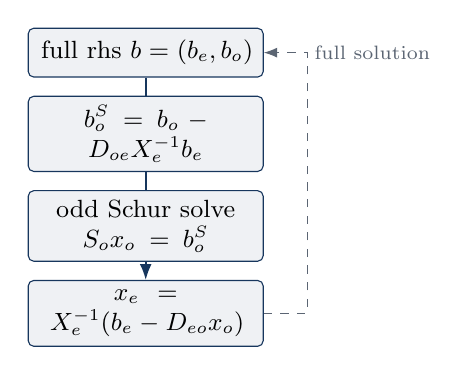
\begin{tikzpicture}[node distance=0.23cm]
        \node[state,text width=2.75cm] (f) {full rhs $b=(b_e,b_o)$};
        \node[state,text width=2.75cm,below=of f] (r) {$b_o^S=b_o-D_{oe}X_e^{-1}b_e$};
        \node[state,text width=2.75cm,below=of r] (s) {odd Schur solve $S_ox_o=b_o^S$};
        \node[state,text width=2.75cm,below=of s] (x) {$x_e=X_e^{-1}(b_e-D_{eo}x_o)$};
        \draw[arrow] (f)--(r)--(s)--(x);
        \draw[relation] (x.east) -- ++(0.55,0) |- node[right=1pt,labelstyle]{full solution} (f.east);
      \end{tikzpicture}
      \vspace{0.2em}
      \begin{alertblock}{实现约束}
        \codepath{use_parity=True} 要求每层已构造 $X/Y$；大格矩阵自由模式关闭 parity，避免隐式 materialize。
      \end{alertblock}
    \end{column}
  \end{columns}
  \source{QUDA：\codepath{multigrid.cpp:1131-1221}；PyQCU：\codepath{_quda_multigrid.py:874-983,1205-1207,1254-1281}。}
\end{frame}

\begin{frame}[t]{V-cycle 与外层 FGMRES：粗解是可变化的右预条件器}
  \footnotesize
  \begin{columns}[T,totalwidth=\textwidth]
    \begin{column}{0.54\textwidth}
      \begin{tabular}{@{}l@{}}
        $x_\ell\leftarrow0$ 或给定初值；\\
        $x_\ell\leftarrow S_{\rm pre}(b_\ell,x_\ell)$；\\
        $r_\ell\leftarrow b_\ell-D_\ell x_\ell$；\\
        $r_{\ell+1}\leftarrow R_\ell r_\ell$；\\
        $e_{\ell+1}\leftarrow\text{recursive coarse solve}(r_{\ell+1})$；\\
        $x_\ell\leftarrow x_\ell+P_\ell e_{\ell+1}$；\\
        $x_\ell\leftarrow S_{\rm post}(b_\ell,x_\ell)$；\\
        $\text{return }K(b_\ell)=x_\ell$。
      \end{tabular}
      \vspace{0.25em}
      \begin{block}{外层}
        \codepath{fgmres(b,D,precond=V-cycle)} 以右预条件形式构造 Arnoldi、复 Givens、上三角回代与 restart；每次 V-cycle 可因残差、层次或粗解精度而变化。
      \end{block}
    \end{column}
    \begin{column}{0.36\textwidth}
      \begin{tikzpicture}[node distance=0.10cm]
        \node[flow,text width=2.25cm,minimum height=0.46cm,font=\scriptsize] (p) {pre-smooth\\消高频};
        \node[flow,text width=2.25cm,minimum height=0.46cm,font=\scriptsize,below=of p] (r) {restrict\\$Rr$};
        \node[flow,text width=2.25cm,minimum height=0.46cm,font=\scriptsize,below=of r] (c) {coarse solve\\递归/底层};
        \node[flow,text width=2.25cm,minimum height=0.46cm,font=\scriptsize,below=of c] (q) {prolongate\\$Pe_c$};
        \node[flow,text width=2.25cm,minimum height=0.46cm,font=\scriptsize,below=of q] (s) {post-smooth\\输出 $K(r)$};
        \draw[arrow] (p)--(r)--(c)--(q)--(s);
      \end{tikzpicture}
      \vspace{0.2em}
      \begin{alertblock}{两种底层}
        \scriptsize
        小格可对显式 coarse matrix 直接 solve；一般情形使用 coarse FGMRES。代码对 zero RHS、zero residual 和 singular breakdown 保持有限值。
      \end{alertblock}
    \end{column}
  \end{columns}
  \source{QUDA：\codepath{multigrid.cpp:1131-1224,564-702}；PyQCU：\codepath{_quda_multigrid.py:1254-1327}、\codepath{_gmres.py:49-156}。}
\end{frame}

\begin{frame}[t]{新旧实现并存：新路径补全代数层，不破坏旧 API}
  \footnotesize
  \begin{center}
    \begin{tabularx}{0.96\textwidth}{@{}P{0.20\textwidth}YY@{}}
      \toprule
      维度 & 旧 \codepath{solver.multigrid} & 新 \codepath{solver.QudaMultigrid} \\
      \midrule
      粗自由度 & flat $E$；接口历史兼容 & $2\times N_{\rm vec}$，显式 coarse spin \\
      transfer & finest/MG-0 有 parity 处理 & 每层共享 map、$V$、$P$、$R=P^\dagger$；含 staggered 1$\to$2 \\
      coarse operator & 33-point/窗口化路径，粗层不是完整 dslash & $D_c=RDP$；materialized block 或 matrix-free composition \\
      Clover/Gauge & 依赖旧粗层约定 & 细层复用 Wilson/Clover dslash；local $X$ 进入每层 Schur \\
      parity & 主要在最细层 & \codepath{ParitySchurOperator} 可作用于任意粗层 \\
      角色 & 历史生产/实验路径，保留 & QUDA 语义的 CPU/CUDA tensor reference \\
      \bottomrule
    \end{tabularx}
  \end{center}
  \vspace{0.10em}
  \begin{block}{兼容策略}
    \scriptsize\codepath{solver/__init__.py} 同时导出旧/新类；测试显式断言二者不是同一类，避免补充实现覆盖旧路径。
  \end{block}
  \source{旧：\codepath{solver/_multigrid.py}；新：\codepath{solver/_quda_multigrid.py:986-1407}；导出/测试：\codepath{solver/__init__.py:1-12}、\codepath{test_quda_multigrid.py:56-58}。}
\end{frame}

\begin{frame}[t]{代数验证结果：核心恒等式与求解 residual 均通过}
  \scriptsize
  \begin{columns}[T,totalwidth=\textwidth]
    \begin{column}{0.49\textwidth}
      \begin{tabular}{@{}P{0.50\linewidth}r@{}}
        \toprule
        指标（$4^4$，c64） & 实测 \\
        \midrule
        多层 $\|RP\eta-\eta\|/\|\eta\|$ & $1.54\times10^{-7}$ \\
        多层 transfer 伴随相对误差 & $5.43\times10^{-9}$ \\
        多层 block Gram 最大误差 & $5.34\times10^{-7}$ \\
        多层 $\|D_c\eta-RD(P\eta)\|/\|RD(P\eta)\|$ & $7.62\times10^{-8}$ \\
        Schur 偶方程重构范数 & $3.18\times10^{-7}$ \\
        \bottomrule
      \end{tabular}
    \end{column}
    \begin{column}{0.41\textwidth}
      \begin{tabular}{@{}P{0.62\linewidth}r@{}}
        \toprule
        求解/边界 & 实测 \\
        \midrule
        多层 full residual & $1.04\times10^{-7}$ \\
        matrix-free residual & $4.07\times10^{-8}$ \\
        staggered $RP$ & $1.41\times10^{-7}$ \\
        staggered 伴随误差 & $9.50\times10^{-9}$ \\
        Wilson Schur even residual & $1.14\times10^{-6}$ \\
        Clover Schur even residual & $2.04\times10^{-6}$ \\
        \bottomrule
      \end{tabular}
      \vspace{0.10em}
      \begin{block}{回归闸门}
        \centering\textbf{9 passed in 6.09s}\par
        覆盖 transfer、Galerkin、$X^{-1}$/Yhat、Schur、多层/单层、lazy、Wilson/Clover+Gauge、staggered 和 FGMRES breakdown。
      \end{block}
    \end{column}
  \end{columns}
  \vspace{0.05em}
  \begin{alertblock}{证据等级}
    以上数值是本次 CPU 小格命令的直接输出；它们证明参考实现的代数约定，不外推 CUDA kernel 的吞吐、MPI scaling 或大格迭代数。
  \end{alertblock}
  \source{命令（在 \codepath{examples/pyqcu}）：\codepath{pytest -q test_quda_multigrid.py}；复核：\codepath{QudaMultigrid.diagnostics()}；测试：\codepath{test_quda_multigrid.py:76-264}。}
\end{frame}

\begin{frame}[t]{关键坑点已变成可回归的不变量，而不是隐含约定}
  \footnotesize
  \begin{center}
    \begin{tabularx}{0.96\textwidth}{@{}P{0.28\textwidth}P{0.34\textwidth}Y@{}}
      \toprule
      发现的边界 & 修复 & 物理/代数后果 \\
      \midrule
      coarse extent $=2$ 时 $+/-$ 邻居相同 & 两方向 block 各折半 & 周期邻居不被 apply 两次 \\
      staggered 延拓把 coarse 坐标误当 fine 展开索引 & 显式按 fine site parity 选 $q$ & 1$\to$2 spin/parity 与 $P/R$ 一致 \\
      backward Yhat 的存储位置/右乘错误 & 移到 $q-\hat\mu$，使用正确 $X^{-\dagger}$ & PC hopping 与 QUDA link convention 对齐 \\
      mixed dtype/device & apply 前转到 $V$ 所在 dtype/device，再转回输入 & CPU/CUDA tensor 接口不因类型漂移失效 \\
      显式 coarse 矩阵内存无上限 & 增加元素上限与 matrix-free 模式 & 大格不因 probe 直接失控；代数仍可 lazy 验证 \\
      zero RHS / singular Arnoldi & FGMRES 提前返回、回代零 pivot 不除零 & V-cycle 的零粗 residual 不产生 NaN \\
      \bottomrule
    \end{tabularx}
  \end{center}
  \vspace{0.10em}
  \begin{block}{工程结论}
    \scriptsize 这些问题来自周期索引、复数伴随、存储位置和奇偶块结构；先固定不变量，再谈 kernel 和性能。
  \end{block}
  \source{修复：\codepath{solver/_quda_multigrid.py:73-88,377-495,657-862}、\codepath{solver/_gmres.py:31-45,77-147}；QUDA：\codepath{coarse_op_preconditioned.cuh:48-120}。}
\end{frame}

\begin{frame}[t,fragile]{可复现入口与当前限制：先用 reference 验证，再迁移到生产后端}
  \footnotesize
  \begin{columns}[T,totalwidth=\textwidth]
    \begin{column}{0.49\textwidth}
      \begin{block}{最小使用形态}
        \begin{lstlisting}[language=Python,aboveskip=0.2em,belowskip=0.2em]
from pyqcu.solver import QudaMultigrid
mg = QudaMultigrid(
    U=U, clover_term=C, kappa=kappa,
    null_vectors=[B0, B1],
    block_size=[(2,2,2,2),(1,1,1,1)],
    max_level=3, use_parity=True)
x = mg.solve(b)
        \end{lstlisting}
        自定义算子则提供 \texttt{fine\_matvec}、\texttt{fine\_diagonal}（启用 parity 时必需）和可选 \texttt{fine\_adjoint}。
      \end{block}
    \end{column}
    \begin{column}{0.41\textwidth}
      \begin{block}{已验证}
        \scriptsize
        \begin{minipage}{0.97\linewidth}
          Python 语法检查；\\[-0.1em]
          CPU 复数单精度 $4^4$；\\[-0.1em]
          Wilson/Clover + Gauge setup；\\[-0.1em]
          staggered transfer 1$\to$2；\\[-0.1em]
          materialized 与 matrix-free；\\[-0.1em]
          旧/新导出并存。
        \end{minipage}
      \end{block}
      \begin{alertblock}{尚未验证}
        \scriptsize
        \begin{minipage}{0.97\linewidth}
          QUDA GPU kernel 的逐项性能等价；\\[-0.1em]
          MPI rank 间 coarse halo/ghost；\\[-0.1em]
          QUDA 的完整 CG/CA-CG/Krylov null setup；\\[-0.1em]
          大格 $L$、混合精度和生产收敛曲线；\\[-0.1em]
          C++ CUDA 后端的直接复用。
        \end{minipage}
      \end{alertblock}
    \end{column}
  \end{columns}
  \vspace{0.05em}
  \begin{center}
    \scriptsize reference 不变量 $\to$ 批量 UV/VUV kernel $\to$ MPI halo $\to$ 全量对照
  \end{center}
  \source{入口：\codepath{solver/_quda_multigrid.py:986-1104,1237-1347}；QUDA 参考：\codepath{coarse_op.cuh}、\codepath{multigrid.cpp}。}
\end{frame}

\begin{frame}[t]{阶段结论：数学复现已闭环，系统复现仍需三步}
  \small
  \begin{columns}[T,totalwidth=\textwidth]
    \begin{column}{0.30\textwidth}
      \begin{block}{主张}
        新实现正确表达了 QUDA 的核心层级对象：\[
          \begin{gathered}
            B\to V\to(P,R)\to RDP\\[-0.2em]
            \to(X,Y)\to\text{Schur/cycle}.
          \end{gathered}
        \]
      \end{block}
      \begin{block}{置信度}
        \verified{} CPU 小格代数验证；\inferred{} 与 QUDA 源码控制流/存储语义相符。
      \end{block}
    \end{column}
    \begin{column}{0.30\textwidth}
      \begin{block}{剩余最大风险}
        参考路径是逐点/逐列 Python 实现；大格 materialization 不可行，matrix-free parity 也有明确约束。生产级性能和通信尚未形成证据。
      \end{block}
      \begin{block}{旧实现定位}
        旧类继续作为历史基线；新类是补全 QUDA 语义的并行实现，不做无声替换。
      \end{block}
    \end{column}
    \begin{column}{0.30\textwidth}
      \begin{block}{下一步可验收产物}
        \scriptsize
        \begin{minipage}{0.97\linewidth}
          1. reference 与 CUDA coarse apply 逐动作等价；\\
          2. 单 rank 再到多 rank halo 回归；\\
          3. 真实 null-vector setup 与大格 residual/性能表。
        \end{minipage}
      \end{block}
      \begin{alertblock}{需要决策}
        是否以本 reference 的不变量作为 CUDA/MPI 迁移的 golden contract；本报告没有性能结论，因此无需据此承诺硬件收益。
      \end{alertblock}
    \end{column}
  \end{columns}
  \source{源码：QUDA 四个核心文件；实现/测试：\codepath{_quda_multigrid.py}、\codepath{test_quda_multigrid.py}。}
\end{frame}

\appendix

\begin{frame}[t]{附录：源码—对象索引与证据等级}
  \scriptsize
  \begin{center}
    \renewcommand{\arraystretch}{0.86}
    \begin{tabularx}{0.96\textwidth}{@{}P{0.25\textwidth}P{0.40\textwidth}Y@{}}
      \toprule
      对象 & QUDA 证据 & PyQCU 证据/状态 \\
      \midrule
      geometry / spin map & \codepath{transfer.cpp:200-257} & \codepath{_quda_multigrid.py}；map、Wilson/Clover 与 staggered \\
      block CGS & \codepath{block_orthogonalize.cuh:149-239} & \codepath{_quda_multigrid.py}；aggregate-local Gram \\
      P / R & \codepath{transfer.cpp:259-328} & \codepath{_quda_multigrid.py}；$R=P^\dagger$ \\
      coarse $X/Y$ & \codepath{coarse_op.cuh:1040-1459} & \codepath{_quda_multigrid.py}；Galerkin $RDP$ \\
      PC / Yhat & \codepath{coarse_op_preconditioned.cuh:48-120} & \codepath{_quda_multigrid.py}；方向/存储 \\
      parity / cycle & \codepath{multigrid.cpp:1131-1224} & \codepath{_quda_multigrid.py}；Schur + FGMRES \\
      生产后端 & CUDA field order、ghost、MPI、MMA、mixed precision & \unverified{}；本任务仅交付 Python reference \\
      \bottomrule
    \end{tabularx}
  \end{center}
  \vspace{0.10em}
  \begin{block}{证据口径}
    \scriptsize\verified{} = 本次命令直接支持；\inferred{} = 由源码结构推出；\unverified{} = 尚未运行或不在范围。数值仅来自 CPU 小格。
  \end{block}
  \source{表中 QUDA 文件相对 \codepath{refer/git-rep/quda}；PyQCU 求解器文件相对 \codepath{pyqcu/solver}；日志 \codepath{logs/v20260829.txt}。}
\end{frame}

\begin{frame}[t]{附录：本次交付清单}
  \small
  \begin{tabular}{@{}l@{}}
    \textbf{实现：}\quad \codepath{pyqcu/solver/_quda_multigrid.py}（新 QUDA 风格参考路径）\\
    \textbf{测试：}\quad \codepath{examples/pyqcu/test_quda_multigrid.py}（9 项 CPU 代数/求解器回归）\\
    \textbf{兼容：}\quad \codepath{pyqcu/solver/__init__.py}、\codepath{pyqcu/cann/__init__.py}\\
    \textbf{稳健性：}\quad \codepath{pyqcu/solver/_gmres.py}（zero RHS 与 breakdown）\\
    \textbf{报告：}\quad \codepath{docs/report_quda_multigrid_reproduction_20260829.tex/.pdf}\\
    \textbf{保留：}\quad 旧 \codepath{pyqcu/solver/_multigrid.py} 未被替换\\
  \end{tabular}
  \vspace{0.45em}
  \begin{center}
    \begin{tikzpicture}[node distance=0.26cm and 0.28cm]
      \node[phase] (q) {QUDA 源码理解};
      \node[phase,right=of q] (p) {Python 代数复现};
      \node[phase,right=of p] (t) {不变量回归};
      \node[phase,right=of t] (n) {CUDA/MPI 迁移};
      \draw[arrow] (q)--(p)--(t)--(n);
      \node[below=0.10cm of n,font=\scriptsize,text=warning] {下一阶段，未包含在本次交付};
    \end{tikzpicture}
  \end{center}
  \source{验证：\codepath{python -m py_compile ...}、\codepath{git diff --check}、\codepath{pytest -q examples/pyqcu/test_quda_multigrid.py}。}
\end{frame}

\end{document}
